\documentclass[11pt]{article}

% ==== PACKAGES ==== %
% \usepackage{fullpage}
\usepackage{amsmath,amssymb,amsthm}
\usepackage{epic}
\usepackage{eepic}
\usepackage{hyperref}
\usepackage{listings}
\usepackage{float}
\usepackage{graphicx}
\usepackage{fancyhdr}
\usepackage{color}
\usepackage{bbm}
\usepackage[letterpaper, margin=1in]{geometry}

% ==== MARGINS ==== %
% \pagestyle{empty}
% \setlength{\oddsidemargin}{0in}
% \setlength{\textwidth}{6.8in}
% \setlength{\textheight}{9.5in}

\pagestyle{fancy}
\fancyhf{}
\rhead{ASEN 5044}
\lhead{Homework 1}
\rfoot{Page \thepage}


\newtheorem*{solution*}{Solution}
\newtheorem{lemma}{Lemma}[section]
\newtheorem{theorem}[lemma]{Theorem}
\newtheorem{claim}[lemma]{Claim}
\newtheorem{definition}[lemma]{Definition}
\newtheorem{corollary}[lemma]{Corollary}
\lstset{moredelim=[is][\bfseries]{[*}{*]}}

% ==== DOCUMENT PROPER ==== %
\begin{document}

\thispagestyle{empty}

% --- Header Box --- %
\newlength{\boxlength}\setlength{\boxlength}{\textwidth}
\addtolength{\boxlength}{-4mm}

\begin{center}\framebox{\parbox{\boxlength}{\bf
      Statistical Estimation \hfill Homework 2\\
      ASEN 5044 Fall 2018 \hfill Due Date: Sep 20, 2018\\
      Name: Andrew Kramer \hfill PhD Student
}}
\end{center}

\section*{Exercise 1}
Consider the 2-mass/3-spring system presented in lecture 4, where the continuous time state definition and inputs are the same, but the observed sensor inputs are now given by 
\begin{equation*}
	y(t) = \begin{bmatrix} 1 & 0 & 0 & 0 \\ 0 & 1 & 0 & -1 \end{bmatrix}x(t) + \begin{bmatrix} 0 & 0 \\ 0 & 0 \end{bmatrix} u(t)
\end{equation*}

\subsection*{Problem (a)}
Find the discrete time LTI representation for this system using a step size of $\Delta T = 0.05$ sec. How does this sampling rate compare with the system's Nyquist limit?

\subparagraph*{}
Recalling lecture 4, the state of the system is given by $x(t) = [q_1(t),\ \dot{q}_1(t),\ q_2(t),\ \dot{q}_2(t)]^T$ where $q_i$ is the displacement of mass $i$ and $u(t) = [u_1(t),\ u_2(t)]^T$ where $u_1$ is the force between the two masses and $u_2$ is the force on mass 2. The CT LTI system model is given by $\dot{x} = Ax(t)+bu(t)$ where
\begin{align*}
	A &= \begin{bmatrix} 0&1.0&0&0 \\ -2.0&0&1.0&0 \\ 0&0&0&1.0 \\ 1.0&0&-2.0&0 \end{bmatrix} \\ 
	B&= \begin{bmatrix} 0&0 \\ -1&0 \\ 0&0 \\ 1&1 \end{bmatrix}
\end{align*}
This is relatively simple to convert to a discrete time system. We only need to find $e^{\hat{A}\Delta t}$ where
\begin{equation*}
	\hat{A} = \begin{bmatrix} 0&1&0&0&0&0 \\ -2&0&1&0&-1&0 \\ 0&0&0&1&0&0 \\ 1&0&-2&0&1&1 \\ 0&0&0&0&0&0 \\ 0&0&0&0&0&0 \end{bmatrix} 
\end{equation*}
The discretized system is described by $x(k+1)=Fx(k)+Gu(k)$ where $F$ is the upper left $4\times 4$ block of $e^{\hat{A}\Delta t}$ and $G$ is the upper right $4\times 2$ block:
\begin{align*}
	F&=\begin{bmatrix}1.0 & 0.05 & 0.001 & 0.0 \\ -0.1 & 1.0 & 0.05 & 0.001 \\ 0.001 & 0.0 & 1.0 & 0.05 \\ 0.05 & 0.001 & -0.1 & 1.0 \end{bmatrix} \\
	G&=\begin{bmatrix} -0.001 & 0.0 \\ -0.05 & 0.0 \\ 0.001 & 0.001 \\ 0.05 & 0.05 \end{bmatrix}
\end{align*}
To satisfy the Nyquist sampling criterion for this system the following inequality must hold $\frac{\pi}{\Delta t} > 2|\lambda_\text{max}|$ where $|\lambda_\text{max}|$ is the largest complex magnitude among all the eigenvalues of $A$. In this case that magnitude is $1.732$. 
\begin{align*}
	\frac{\pi}{\Delta t} &= 62.83 \\
	2|\lambda_\text{max}| &= 3.464
\end{align*}
Clearly in this case the sampling frequency is well within the Nyquist limit for this system.

\subsection*{Problem (b)}
Show that the DT system is observable.

\subparagraph*{}
We'll start by building candidates for our observability matrix $\mathbb{O}$ and checking if they are full rank. The simplest possible case, $\mathbb{O} = H$ is rank deficient, because column $4$ of $H$ is simply column $2$ multiplied by $-1$.
\begin{equation*}
	H = \begin{bmatrix} 1 & 0 & 0 & 0 \\ 0 & 1 & 0 & -1 \end{bmatrix}
\end{equation*}
The next possibility, $[H,\ HF]^T$, is full rank. 
\begin{equation*}
	\mathbb{O} = \begin{bmatrix} H \\ HF \end{bmatrix} = \begin{bmatrix} 1.0 & 0.0 & 0.0 & 0.0 \\ 0.0 & 1.0 & 0.0 & -1.0 \\ 1.0 & 0.05 & 0.001 & 0.0 \\ -0.15 & 1.0 & 0.15 & -1.0 \end{bmatrix}
\end{equation*}
This means the system is fully observable from two observations. This makes physical sense, as the displacement of mass 1, $x_1$ is directly measurable (as $y_1$) so we should be able to find the velocity of mass 1, $x_2$ with two measurements of its position. Then, if we know velocity of mass 1 and the relative velocity of the two masses, $y_2$ it is possible to calculate the velocity of mass 2, $x_4$. Lastly, knowing the velocity of mass 2 over one timestep will also allow us to calculate its displacement $x_3$ over that timestep.

\subsection*{Problem (c)}
Suppose the system starts from some unknown initial condition $x(0)$ at $k=0$ and is stimulated by an external set of ZOH inputs $u$ at the $\Delta T = 0.05$ sec sampling rate from $t=0$ to $t=5$ seconds, where $u(t)=[\sin(t), 0.1\cos(t)]^T$, and the resulting output $y(k)$ at each sampling instant from $t=0.05$ sec ($k=1$) to $t=5$ sec is recorded in \texttt{hw3problemdata.mat}. Derive a linear system of equations in matrix-vector form that would allow you to estimate the unknown initial condition $x(k=0)$ using all the available logged $y$ and $u$ data.

\subparagraph*{}
We can regress $x(0)$ from the logged $n$ measurements by stacking the measurements to form an $np\times1$ column vector $Y$ which will follow the relationship
\begin{equation*}
	Y = \mathbb{O}x(0)
\end{equation*}
where $\mathbb{O}=[HF^0,\ HF^1,\ HF^2,\ \dots, HF^{n-1}]^T$. We can solve for $x(0)$ by multiplying both sides by the grammian of $\mathbb{O}$:
\begin{equation*}
	x(0) = (\mathbb{O}^T\mathbb{O})^{-1}\mathbb{O}^TY
\end{equation*}

THE ABOVE ONLY HOLDS FOR SYSTEMS WITH NO INPUT!

\subsection*{Problem (d)}
Estimate $x(k=0)$ and plot all the remaining states $x(k)$ for $k\geq 1$ vs time (in seconds) and separately plot their corresponding 'predicted' outputs $y(k)$ vs. time for all $k\geq 1$ in the recorded output time series. Validate your estimate by also separately plotting the differences between the 'predicted' and recorded $y(k)$ values vs. time.

\subparagraph*{}
In solving $(\mathbb{O}^T\mathbb{O})^{-1}\mathbb{O}^TY$ we find that $x(0)=[0.247,\ 0.434,\ -0.607,\ -1.697]$. See figure \ref{fig:1d_states} below for a plot of the predicted states vs. time and figure \ref{fig:1d_meas} for the predicted outputs. Figure \ref{fig:1d_diffs} shows the difference between the predicted and actual measurements. The predicted measurements match the actual measurements exactly in frequency, though their amplitude differs.

\begin{figure}[h!]
	\centering
	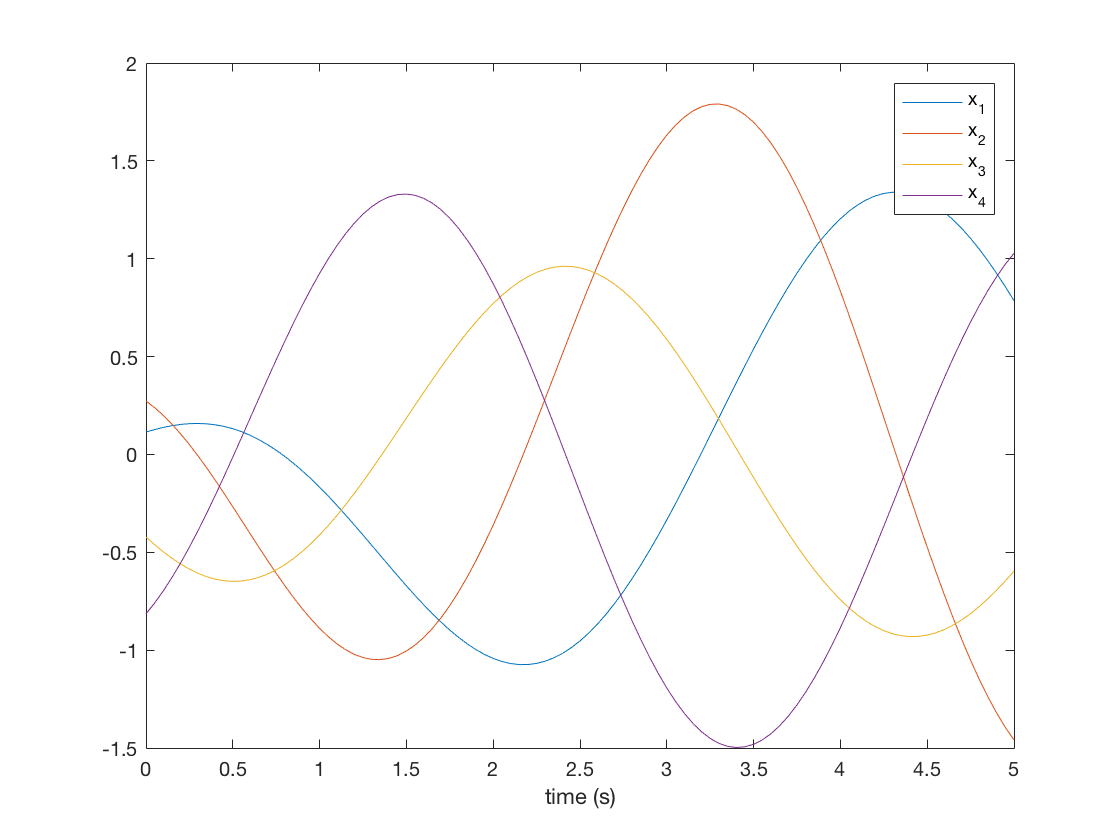
\includegraphics[width=0.6\linewidth]{1d_state_plot.png}
	\caption{predicted states}
	\label{fig:1d_states}
\end{figure}
\begin{figure}[h!]
	\centering
	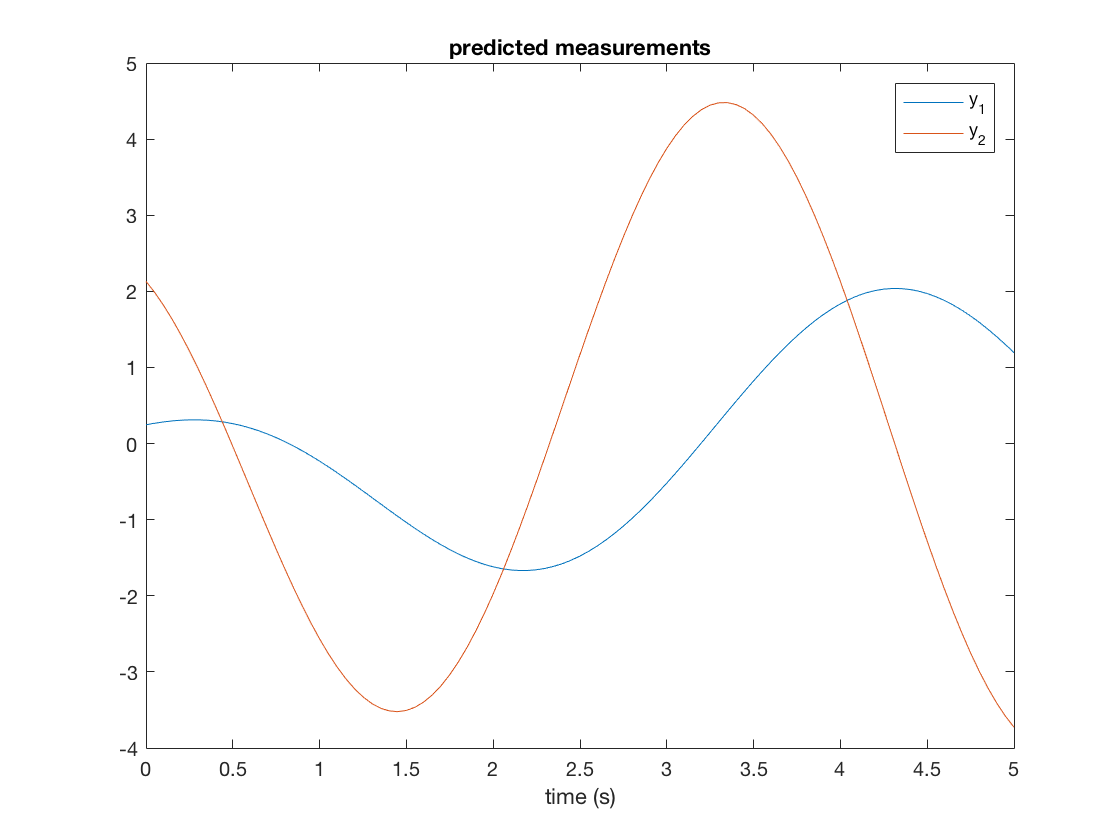
\includegraphics[width=0.6\linewidth]{1d_pred_meas.png}
	\caption{predicted measurements}
	\label{fig:1d_meas}
\end{figure}
\begin{figure}[h!]
	\centering
	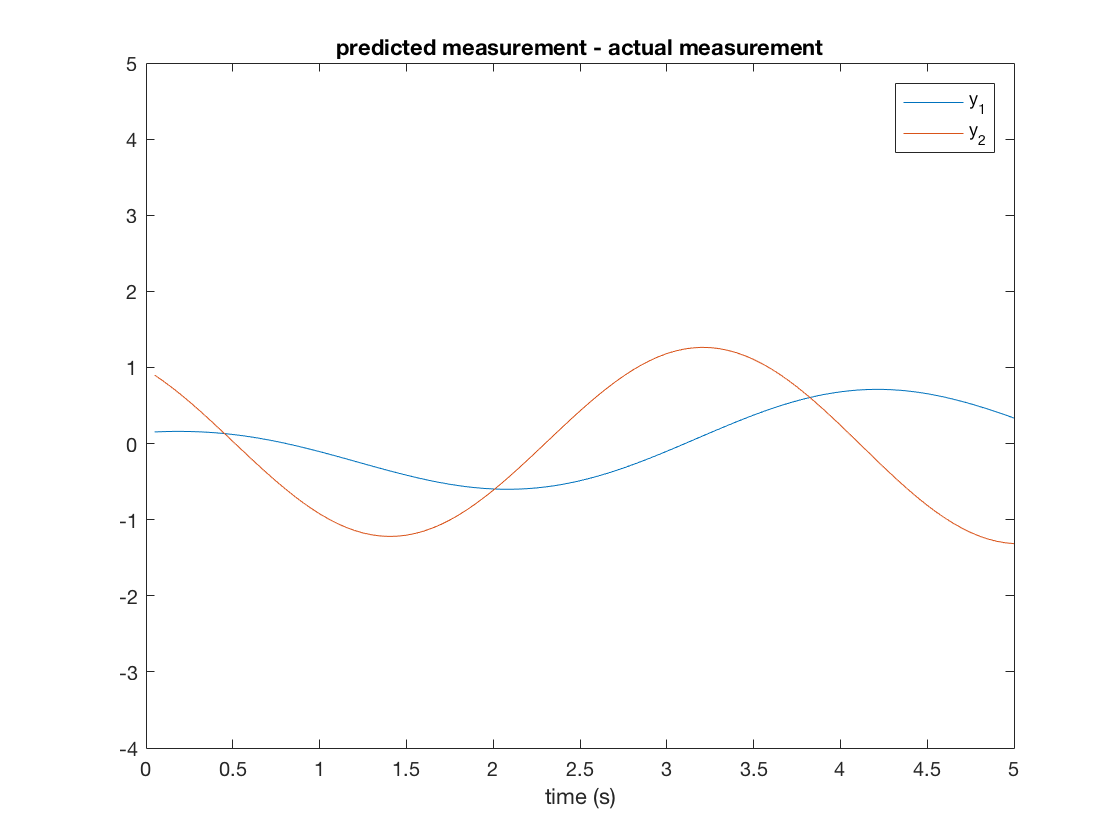
\includegraphics[width=0.6\linewidth]{1d_meas_diffs.png}
	\caption{difference between predicted and actual measurements}
	\label{fig:1d_diffs}
\end{figure}

\subsection*{Problem (e)}
How many vector measurements $y(k)$ are actually needed to estimate $x(0)$, i.e. do you need to use all available measurements, or some smaller number? Is this consistent with an analysis of the observability matrix $\mathbb{O}$ and Grammian $\mathbb{O}^T\mathbb{O}$? Explain how and why the required number of vector measurements would theoretically change if the $y(k)$ data were instead given by three different position sensors for the first mass, where 
\begin{equation*}
	H=\begin{bmatrix} 1&0&0&0 \\ 1&0&0&0 \\ 1&0&0&0 \end{bmatrix}
\end{equation*}

\subparagraph*{}

\subsection*{Problem (f)}
What happens to the observability of the system if only the first row of the output $y(k)$ is used for all $k\geq 1$? What if only the second row of the output vector $y(k)$ is used instead? Provide a physical explanation in each case.

\end{document}
